% !TEX program = xelatex
\documentclass[10pt,a4paper,oneside]{article}
\usepackage[utf8]{inputenc}
\usepackage[vietnamese]{babel}
\usepackage{fontspec}
\usepackage{geometry}
\usepackage{xcolor}
\usepackage{tikz}
\usepackage{graphicx}
\usepackage{tabularx}
\usepackage{booktabs}
\usepackage{array}
\usepackage{multicol}
\usepackage{enumitem}
\usepackage{microtype}
\usepackage{fancyhdr}
\usepackage{fontawesome5}

\usetikzlibrary{shapes.geometric, arrows.meta, positioning, calc, backgrounds, shadows, fit}

% Set margins: 12mm left/right, 14mm top, 14mm bottom
\geometry{a4paper, top=14mm, bottom=14mm, left=12mm, right=12mm, headheight=0mm, headsep=0mm, footskip=0mm}

% Typography: Segoe UI with robust fallback
\IfFontExistsTF{Segoe UI}{
  \setmainfont{Segoe UI}[
    BoldFont={Segoe UI Bold},
    ItalicFont={Segoe UI Italic},
    BoldItalicFont={Segoe UI Bold Italic}
  ]
}{
  \IfFontExistsTF{Arial}{
    \setmainfont{Arial}[
      BoldFont={Arial Bold},
      ItalicFont={Arial Italic},
      BoldItalicFont={Arial Bold Italic}
    ]
  }{
    \setmainfont{DejaVu Sans}[
      BoldFont={DejaVu Sans Bold},
      ItalicFont={DejaVu Sans Oblique},
      BoldItalicFont={DejaVu Sans Bold Oblique}
    ]
  }
}

% Color Palette - Luxury Corporate High-Tech
\definecolor{TTCDeepNavy}{RGB}{10, 25, 47}
\definecolor{TTCBlue}{RGB}{15, 60, 120}
\definecolor{TTCLightBlue}{RGB}{240, 246, 255}
\definecolor{TTCRed}{RGB}{214, 40, 40}
\definecolor{TTCCyan}{RGB}{0, 180, 216}
\definecolor{TTCGold}{RGB}{247, 127, 0}
\definecolor{TTCTextDark}{RGB}{30, 41, 59}
\definecolor{TTCTextMuted}{RGB}{100, 116, 139}
\definecolor{TTCBorder}{RGB}{203, 213, 225}

\newcolumntype{Y}{>{\centering\arraybackslash}X}
\newcolumntype{L}{>{\raggedright\arraybackslash}X}
\newcolumntype{R}{>{\raggedleft\arraybackslash}X}

\setlength{\parindent}{0pt}
\setlength{\parskip}{0pt}
\linespread{1.05}
\pagestyle{empty}

% Header & Footer Macros
\newcommand{\pageheaderbar}[2]{%
  \begin{tikzpicture}[remember picture, overlay]
    \fill[TTCDeepNavy] (current page.north west) rectangle ([yshift=-10mm]current page.north east);
    \fill[TTCRed] ([yshift=-10mm]current page.north west) rectangle ([yshift=-11mm]current page.north east);
    \node[anchor=west, text=white, font=\fontsize{7.5}{9}\selectfont\bfseries] at ([xshift=12mm, yshift=-5mm]current page.north west) {
      \faBuilding\quad CÔNG TY CỔ PHẦN CÔNG NGHỆ XÂY DỰNG TÂN THÀNH CÔNG \textbullet\ TTC JSC
    };
    \node[anchor=east, text=TTCCyan, font=\fontsize{7.5}{9}\selectfont\bfseries] at ([xshift=-12mm, yshift=-5mm]current page.north east) {
      #1
    };
  \end{tikzpicture}%
}

\newcommand{\pagefooterbar}[1]{%
  \begin{tikzpicture}[remember picture, overlay]
    \fill[TTCDeepNavy] (current page.south west) rectangle ([yshift=8mm]current page.south east);
    \fill[TTCCyan] ([yshift=8mm]current page.south west) rectangle ([yshift=8.8mm]current page.south east);
    \node[anchor=west, text=white, font=\fontsize{6.8}{8}\selectfont] at ([xshift=12mm, yshift=4mm]current page.south west) {
      \faPhone*\ +84 976 447 766 \quad\textbullet\quad \faEnvelope\ info@tanthanhcongjsc.com \quad\textbullet\quad \faGlobe\ https://tanthanhcongjsc.com
    };
    \node[anchor=east, text=white, font=\fontsize{7}{8}\selectfont\bfseries] at ([xshift=-12mm, yshift=4mm]current page.south east) {
      #1
    };
  \end{tikzpicture}%
}

% Section Header Brand Macro
\newcommand{\secbrand}[2]{%
  \noindent\begin{tikzpicture}
    \fill[TTCRed] (0,0) rectangle (4mm,10mm);
    \node[anchor=west, align=left, inner sep=0pt] at (6mm, 5mm) {
      {\fontsize{13}{15}\selectfont\bfseries\color{TTCBlue} #1}\\[1.5pt]
      {\fontsize{7.2}{8.8}\selectfont\itshape\color{TTCTextMuted} #2}
    };
  \end{tikzpicture}\par\vspace{1.5mm}%
}

\begin{document}
% ============================================================
% TRANG 24: CASE STUDY 03 -- TỔ HỢP JAPFA COMFEED [TRANG MỚI TÁCH RIÊNG]
% ============================================================
\pageheaderbar{SELECTED CASE STUDY 03 -- JAPFA COMFEED COMPLEX}{Trang 24}
\pagefooterbar{Trang 24}

\begin{tikzpicture}[remember picture, overlay]
  \node[opacity=0.03, scale=2.8, font=\bfseries\sffamily, text=TTCBlue] at ([yshift=-10mm]current page.center) {JAPFA COMFEED AGRO-INDUSTRIAL COMPLEX};
  \draw[TTCBlue!6!white, line width=0.5pt] ([xshift=15mm, yshift=20mm]current page.south west) grid[step=8mm] ([xshift=195mm, yshift=45mm]current page.south west);
\end{tikzpicture}

\begin{minipage}[t][246mm]{\textwidth}
\secbrand{Case Study 03: Tổ Hợp Nhà Máy Thức Ăn Chăn Nuôi Japfa Comfeed}{Japfa Comfeed Agro-Industrial Complex \textbullet\ 50,000 m$^2$ \textbullet\ 45m Silo Tower \textbullet\ Heavy Dynamic Load Foundations}

% TẦNG 1: ẢNH HIỆN TRƯỜNG DỰ ÁN (Trái) \& THÔNG SỐ KỸ THUẬT (Phải)
\noindent
\begin{tabular}{@{}p{100mm}@{\hspace{4mm}}p{82mm}@{}}
  % Ảnh dự án
  \begin{tikzpicture}
    \clip[rounded corners=6pt] (0,0) rectangle (10.0, 9.2);
    \node[anchor=center, inner sep=0pt] at (5.0, 4.6) {
      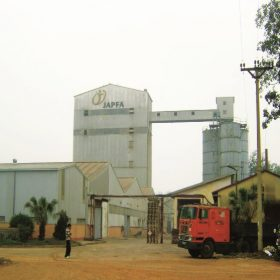
\includegraphics[width=100mm, height=92mm]{../../public/project-assets/japfa.jpg}
    };
    \fill[TTCDeepNavy, opacity=0.85] (0, 0) rectangle (10.0, 1.4);
    \node[anchor=west, text=white, font=\fontsize{7.5}{9}\selectfont\bfseries] at (0.3, 0.7) {
      \faIndustry\quad TỔ HỢP NHÀ MÁY JAPFA COMFEED -- VĨNH PHÚC / THÁI BÌNH
    };
  \end{tikzpicture} &
  % Thông số kỹ thuật
  \begin{tikzpicture}
    \node[
      rounded corners=6pt,
      fill=TTCDeepNavy!95!black,
      draw=TTCCyan!80!white,
      line width=0.9pt,
      minimum width=82mm,
      minimum height=92mm,
      inner sep=6pt,
      text width=74mm,
      align=left
    ] {
      {\fontsize{8.8}{10.8}\selectfont\bfseries\color{TTCCyan} \faInfoCircle\quad THÔNG TIN TỔNG QUAN DỰ ÁN:}\\[4pt]
      {\fontsize{7.2}{9.5}\selectfont\color{white}
      \textbf{Chủ đầu tư:} Tập đoàn Japfa Comfeed (Indonesia)\newline
      \textbf{Địa điểm:} Tỉnh Vĩnh Phúc \& Tỉnh Thái Bình\newline
      \textbf{Diện tích quy hoạch:} \textbf{\color{TTCGold}50.000 m$^2$}\newline
      \textbf{Chiều cao tháp Silo:} \textbf{\color{TTCCyan}45 mét (Kết cấu thép Silo)}\newline
      \textbf{Khối lượng kết cấu thép:} \textbf{\color{white}2.800 Tấn PEB}\newline
      \textbf{Thời gian thi công:} \textbf{\color{TTCRed}165 ngày (Fast-track)}\newline
      \textbf{Tiêu chuẩn an toàn:} \textbf{OHSAS 18001 / HACCP}\newline
      \textbf{Phạm vi hợp đồng:} Tổng thầu EPC Xây dựng xưởng sản xuất cám, cụm tháp Silo chứa ngũ cốc 45m, móng sâu chịu động lực máy nghiền \& Trạm điện 22kV.}\\[6pt]
      \rule{\linewidth}{0.4pt}\\[4pt]
      {\fontsize{6.8}{8.5}\selectfont\color{white!80!gray}
      Dự án vốn FDI Indonesia đạt chuẩn quốc tế khắt khe về an toàn thực phẩm, chống nổ bụi và vận hành liên tục 24/7.}
    };
  \end{tikzpicture}
\end{tabular}

\vspace{2mm}

% TẦNG 2: 3 ĐIỂM NỔI BẬT KỸ THUẬT
\noindent
\begin{tabular}{@{}p{59mm}@{\hspace{3.5mm}}p{59mm}@{\hspace{3.5mm}}p{59mm}@{}}
  \begin{tikzpicture}
    \node[rounded corners=4pt, fill=TTCLightBlue, draw=TTCBorder, line width=0.6pt, minimum width=59mm, minimum height=50mm, inner sep=4pt, text width=53mm, align=left] {
      {\fontsize{8}{9.5}\selectfont\bfseries\color{TTCRed} \faBuilding\ Tháp Silo Kết Cấu Cao 45m}\\[2pt]
      {\fontsize{6.5}{8}\selectfont\color{TTCTextDark}
      \textbullet\ Thi công lắp dựng tháp Silo thép cao 45m an toàn tuyệt đối.\newline
      \textbullet\ Sử dụng cẩu 100T tự hành lắp dựng các phân đoạn siêu trọng.\newline
      \textbullet\ Kiểm tra 100\% bu-lông cường độ cao 10.9 bằng cờ lê lực.}
    };
  \end{tikzpicture} &
  \begin{tikzpicture}
    \node[rounded corners=4pt, fill=TTCLightBlue, draw=TTCBorder, line width=0.6pt, minimum width=59mm, minimum height=50mm, inner sep=4pt, text width=53mm, align=left] {
      {\fontsize{8}{9.5}\selectfont\bfseries\color{TTCCyan} \faShield*\ Chống Nổ Bụi & Thông Gió}\\[2pt]
      {\fontsize{6.5}{8}\selectfont\color{TTCTextDark}
      \textbullet\ Thiết kế hệ thống thu gom và lọc bụi túi vải đạt chuẩn ATEX.\newline
      \textbullet\ Cửa xả áp lực nổ tự động trên mái và vách tháp Silo.\newline
      \textbullet\ Đảm bảo môi trường làm việc sạch bụi đạt chuẩn HACCP.}
    };
  \end{tikzpicture} &
  \begin{tikzpicture}
    \node[rounded corners=4pt, fill=TTCLightBlue, draw=TTCBorder, line width=0.6pt, minimum width=59mm, minimum height=50mm, inner sep=4pt, text width=53mm, align=left] {
      {\fontsize{8}{9.5}\selectfont\bfseries\color{TTCBlue} \faHammer\ Móng Chịu Tải Động Lực}\\[2pt]
      {\fontsize{6.5}{8}\selectfont\color{TTCTextDark}
      \textbullet\ Móng cọc khoan nhồi sâu D800 chịu tải trọng động máy nghiền.\newline
      \textbullet\ Đệm cao su giảm chấn triệt tiêu rung động lan truyền.\newline
      \textbullet\ Đổ bê tông khối lớn liên tục không để lại mạch ngừng nhiệt.}
    };
  \end{tikzpicture}
\end{tabular}

\vspace{2mm}

% TẦNG 3: BĂNG KPI CASE STUDY 3
\noindent
\begin{tikzpicture}
  \node[
    rounded corners=6pt,
    fill=TTCDeepNavy!95!black,
    draw=TTCCyan!80!white,
    line width=1pt,
    text=white,
    minimum width=186mm,
    minimum height=20mm,
    inner sep=4pt
  ] {
    \begin{tabularx}{176mm}{@{}Y|Y|Y|Y@{}}
      {\fontsize{14}{16}\selectfont\bfseries\color{TTCRed} 50.000 m$^2$} &
      {\fontsize{14}{16}\selectfont\bfseries\color{TTCCyan} SILO 45M} &
      {\fontsize{14}{16}\selectfont\bfseries\color{white} 2.800 TẤN} &
      {\fontsize{14}{16}\selectfont\bfseries\color{TTCGold} 0 SỰ CỐ} \\
      {\fontsize{7.2}{9}\selectfont Diện Tích Quy Hoạch} &
      {\fontsize{7.2}{9}\selectfont Chiều Cao Tháp Thép} &
      {\fontsize{7.2}{9}\selectfont Khối Lượng Thép PEB} &
      {\fontsize{7.2}{9}\selectfont An Toàn Tuyệt Đối}
    \end{tabularx}
  };
\end{tikzpicture}
\end{minipage}
\newpage

\end{document}
